\section{Examples}\label{sec:examples}

\subsection{Simple Examples}

Returning to our example programs in \autoref{sec:intro}, after running them through the size inference algorithm, their types in limit \lang are:

\begin{minted}[escapeinside=<>,mathescape=true]{coq}
Def minus: Nat<$^\iota$> <$\to$ >Nat<$^\iota$> <$\to$> Nat<$^\iota$> <$\coloneqq$> <$\dots$>.
Def div: Nat<$^\iota$> <$\to$ > Nat<$^\infty$> <$\to$> Nat<$^\iota$> <$\coloneqq$> <$\dots$>.
\end{minted}

The body of \texttt{div} only needs to know that \texttt{minus} has type $\text{Nat}^\iota \to \text{Nat}^\iota \to \text{Nat}^\iota$ and nothing else.
Furthermore, we have no problems using variables in our fixpoint types (note that we use 1-based indexing):

\begin{minted}[escapeinside=<>,mathescape=true]{coq}
Def aNat: Set <$\coloneqq$> Nat<$^\infty$>.
Def add: aNat<$^{\langle\iota\rangle}$> <$\to$> aNat<$^{\langle\infty\rangle}$> <$\to$> aNat<$^{\langle\infty\rangle}$> <$\coloneqq$>
  fix<$_{\langle 1 \rangle, 1}$> add': aNat<$^{\langle * \rangle}$> <$\to$> Nat <$\to$> Nat <$\coloneqq$> <$\dots$>.
\end{minted}

For the following examples we use a more succinct, Coq-like syntax for brevity, adding in size-inferred global annotations where necessary, and omitting $\infty$ annotations for clarity.
Assuming the usual definition for \text{List}s and \text{Bool}s and if--then--else syntactic sugar for matching on Bools, we can construct a \texttt{filter} function with size-preserving types, since the output list is never longer than the input list.

\begin{minted}[escapeinside=<>,mathescape=true]{coq}
Definition filter:
  (A: Set) -> (A -> Bool) -> List<$^\iota$> A -> List<$^\iota$> A :=
  fix filter' A pred (l: List<$^*$> A): List<$^*$> A :=
    match l with
      | Nil => Nil
      | Cons _ hd tl =>
        if pred hd
        then Cons A hd (filter' A pred tl)
        else (filter' tl)
    end.
\end{minted}

We also have an \texttt{append} function that is \textit{not} size-preserving.
\begin{minted}[escapeinside=<>,mathescape=true]{coq}
Definition append:
  (A: Set) -> List<$^\iota$> A -> List A -> List A := <$\dots$>.
\end{minted}

Now we are all set to implement \texttt{quicksort} on \texttt{Nat}s:
\begin{minted}[escapeinside=<>,mathescape=true]{coq}
Definition quicksort:
  (A: Set) -> List<$^\iota$> Nat -> List Nat :=
  fix quicksort' A (l: List<$^*$> Nat): List Nat :=
    match l with
    | Nil => Nil
    | Cons _ hd tl => append A
      (quicksort' (filter Nat (gtb hd) tl))
      (Cons Nat hd
        (quicksort' (filter Nat (leb hd) tl)))
    end.
\end{minted}
Even though the output list has the same length as the input list, there is no way to add sizes in our current size algebra, so the return type of \texttt{append} is not annotated with the same size as the input type of \texttt{quicksort}. While asserting that \texttt{quicksort} does not change the length of the list requires additional proof, the fact that it \textit{terminates} is given to us by virtue of being typeable.

On the other hand, it is because we cannot express any size relations more complicated than size-preservation that \texttt{gcd}, while terminating, is not typeable.

\begin{minted}[escapeinside=<>,mathescape=true]{coq}
Definition modulo: Nat -> Nat<$^\iota$> -> Nat<$^\iota$> := <$\dots$>
Fail Definition gcd: Nat -> Nat -> Nat :=
  fix gcd' a b :=
    match a with
    | O => b
    | S a' => gcd' (modulo b a) a
    end.
\end{minted}

Because \texttt{modulo} can only determine that the return type is at most as large as its second argument, the first argument to the recursive call in \texttt{gcd'} has a type with the same size as \texttt{a}, and is not deemed to decrease on its first argument.

In the implementation in Coq, programs that type check only with sized types can be declared by first turning off guard checking using the existing flag, then turning on sized typing.

\begin{minted}{coq}
Unset Guard Checking.
Set Sized Typing.
\end{minted}

This way, we can type check either (1) programs that type check only with sized types, or (2) programs that type check only with guard checking.
Note that in the implementation, we do not annotate the types ourselves; any annotations seen in the examples in this section are inferred.

\subsection{Non-Typeable Programs}
Evidently, not every terminating program will type check.
However, there are some classes of non-typeable programs worth describing, as their non-typeability stems from implementation details.

\subsubsection{Successor-Sized (Co)recursive Arguments}
Consider the following rather vacuous example:

\begin{minted}{coq}
Fail Fixpoint vacuous n :=
  match n with
  | O => O
  | S n' => vacuous O
  end.
\end{minted}

When called, this function would always terminate with O, but it does not type check.
This is due to the first step of \RecCheck.
Suppose $\text{O}: \text{Nat}^{\hat{s}}$ and suppose the recursive argument type's position size annotation is $\tau$. 
By \refrule{a-app}, \texttt{vacuous O} would produce the constraint $\hat{s} \sqsubseteq \tau$.
In \RecCheck, we let $\tau$ subsize each size variable in its downward closure, which includes $s$, yielding the constraint $\tau \sqsubseteq s$.
Since this produces a negative cycle that includes $\tau$, \RecCheck fails.

However, we cannot simply remove the first step, since this would allow nonterminating behaviour, as in the example below.

\begin{minted}{coq}
Fail Fixpoint loop n :=
  match n with
  | O => loop O
  | S n' => O
  end.
\end{minted}

Note that these would also fail under guard checking, since O is not a syntactically-smaller element of $n$.

\subsubsection{Local Size Non-Preservation}
Recall that in \RecCheckLoop, $V_{\text{outer}}$ corresponds to the size variables used outside of a \cofixpoint.
They are then passed to the $V^{\neq}$ argument of \RecCheck, which essentially forces those size variable to be infinite.
This has the curious effect of destroying size-preservation when a local definition is outside of a fixpoint, but not when it is inside:

\begin{minted}{coq}
Fail Definition outside :=
  let id x := x in
  fix f n :=
    match n with
    | O => O
    | S n' => f (id n')
    end.
Definition inside :=
  fix f n :=
    let id x := x in
    match n with
    | O => O
    | S n' => f (id n')
    end.
\end{minted}

In \texttt{outside}, \texttt{id} would have type $\text{Nat}^\infty \to \text{Nat}^\infty$, which means that the size of the argument to the recursive call to \texttt{f} is infinite.
In \texttt{inside}, rewriting the let-in in bare \lang as $\letin{\text{id}}{\text{Nat} \to \text{Nat}}{\abs{x}{\text{Nat}}{x}}{\dots}$, the lambda would have type $\text{Nat}^{s} \to \text{Nat}^{s}$, while \texttt{id} has type $\text{Nat}^{s_1} \to \text{Nat}^{s_2}$ for some size expressions $s, s_1, s_2$.
Furthermore, $\text{Nat}^{s} \to \text{Nat}^{s} \leq \text{Nat}^{s_1} \to \text{Nat}^{s_2}$ also yields the subsizing constraints $s_1 \sqsubseteq s \sqsubseteq s_2$.
Then the size of argument to the recursive call to \texttt{f} is $s_2$, which in this case is not infinite.

Notice that due to the subsizing relation $s_1 \sqsubseteq s_2$, there is a relationship between the size of \texttt{n'} and the size of the argument to \texttt{f}. The reason we need to set outer size variables to infinite is because the constraint equivalent to $s_1 \sqsubseteq s_2$ arising from \texttt{id} in the \texttt{outside} case is not passed to the size inference algorithm when checking the fixpoint.
In general, constraints generated outside of a term are not passed to the algorithm when checking that term.
This is clearly at odds with the formal presentation we have provided, which means I need to quickly go fix the implementation now.

\subsubsection{Unpreserved Sizes}

Global definitions of \cofixpoints can be typed to be size-preserving, while other global definitions cannot.
This is because the position size variables of \cofixpoints yield global annotations in the definition types, while other global definition types only have infinite annotations.
This means that some non-\cofixpoint functions we expect to be size-preserving are not, and if we use them as a helper function in a \cofixpoint, it will no longer type check.
The following is an example with the identity function (on naturals) with type $\text{Nat}^\infty \to \text{Nat}^\infty$ used inside a recursive call:

\begin{comment}
A fixpoint must have at one recursive argument -- that is, in the call to that fixpoint in its body, the size of that argument must decrease.
If the return type has the same type as that argument, and the object returned has the same size as the argument, then the return type would have the same size as the argument type, and the size is preserved.
The argument is similar for cofixpoints: the returned object must have a larger size than that returned by the call to the cofixpoint, and if an argument has the same type and size, then the size is preserved.

Aside from global \cofixpoints, local definitions of functions may be size-preserving as well, since the constraints generated from those local definitions are passed to the size inference algorithm when checking a \cofixpoint.
However, global non-\cofixpoint definitions are always assigned infinite size annotations; otherwise, all functions would have to be considered as possibly size-preserving.
This is particularly challenging, as multivariable functions in Coq are in reality curried single-variable abstractions in \lang.
Furthermore, the benefit of size-preserved functions is to allow termination checking of certain \cofixpoints, such as \texttt{quicksort} above, and there generally is no reason for a function to be size-preserving if it were not a \cofixpoint in the first place.
The consequence of this is that using functions in \cofixpoints where size-preservation is expected leads to failure of type checking, such as in the following example.
\end{comment}

\begin{minted}{coq}
Definition id (n: Nat) := n.
Fail Fixpoint f (n: Nat) :=
  match n with
  | O => O
  | S n' => f (id n')
  end.
\end{minted}

A simple workaround is to define \texttt{id} as a fixpoint, which would make it trivially size-preserving.
Alternatively, and perhaps less ideally for larger functions, we could define \texttt{id} within the body of the fixpoint so that it is within the size inference scope of the fixpoint.
\begin{multicols}{2}
\begin{minted}{coq}
Fixpoint id (n: Nat) := n.
Fixpoint f (n: Nat) :=
  match n with
  | O => O
  | S n' => f (id n')
  end.
\end{minted}
\begin{minted}{coq}
Fixpoint g (n: Nat) :=
  let id (m: Nat) := m in
  match n with
  | O => O
  | S n' => g (id n')
  end.
\end{minted}
\end{multicols}

We cannot simply assign new size variables to the type of \texttt{id}, since size inference and constraint generation is done independently for each global declaration, and we have no information on how these new size variables relate to each other inside other declarations.

To truly make global definitions of functions size-preserving, the type system of \lang would have to be adjusted to accommodate additional position annotations and size variables, and the size inference algorithm would have to run \RecCheck for global definitions.
Alternatively, Coq's unfolding mechanism from guard checking could be incorporated into the size inference algorithm.

\subsection{Size Inference Walkthrough}
In this subsection, we present a walkthrough of the size inference algorithm and the generated constraints of the following simple but nontrivial bare \lang program:

\begin{minted}[escapeinside=<>,mathescape=true]{coq}
Def example: Nat <$\to$> Nat <$\coloneqq$>
  fix<$_{\langle 1 \rangle, 1}$> <$\langle$>f: Nat <$\to$> Nat <$\coloneqq$>
    <$\lambda$>n: Nat. case<$_{\lambda x: \texttt{Nat}. \texttt{Nat}}$> n of
      <$\langle$>O <$\Rightarrow$> O,
       S <$\Rightarrow$> <$\lambda$>n': Nat. f n'<$\rangle \rangle$>.
\end{minted}

For convenience, we refer to the definition body, the fixpoint body, and the abstraction body as \texttt{defBody}, \texttt{fixBody}, and \texttt{absBody}, respectively.
We omit reasonably simple steps and examine terms not necessarily in the same order as the algorithm, so the numbering on the size variables may differ from what the implementation yields.

We begin with \refrule{a-global-def}, annotating the definition type as $\text{Nat}^{\upsilon_1} \to \text{Nat}^{\upsilon_2}$.
Inference on \texttt{defBody} takes us to \refrule{a-fix}, where the fixpoint type with position annotations becomes $\text{Nat}^{\tau_1} \to \text{Nat}^{\tau_2}$.
Inference on \texttt{fixBody} takes us to \refrule{a-abs}, where $n$ gets type $\text{Nat}^{\upsilon_3}$.
Finally, inference on \texttt{absBody} takes us to \refrule{a-case}.

Inference on various parts of the case expression gives us the following (recalling that the argument type of abstractions are unannotated):
\begin{itemize}
    \item The target is $n: \text{Nat}^{\upsilon_3}$;
    \item The motive becomes $\abs{x}{\text{Nat}}{\text{Nat}^{\upsilon_5}} : \text{Nat}^{\upsilon_4} \to \Set$;
    \item The first branch is $\text{O}: \text{Nat}^{\upsilon_6}$; and
    \item The second branch is $\abs{n'}{\text{Nat}}{f n'} : \text{Nat}^{\upsilon_7} \to \text{Nat}^{\tau_2}$.
\end{itemize}

Meanwhile, we also compute the expected types of these parts:
\begin{itemize}
    \item \casesize tells us the expected type of the target should have size annotation $\hat{\upsilon}_8$;
    \item \motivetype yields $\text{Nat}^{\hat{\upsilon}_8} \to \Set$;
    \item \branchtype for the first branch yields an application of the motive which reduces to $\text{Nat}^{\upsilon_5}$; and
    \item \branchtype for the second branch yields a similar type that reduces to $\text{Nat}^{\upsilon_8} \to \text{Nat}^{\upsilon_5}$.
\end{itemize}

Travelling back out, we have that $\texttt{absBody}: \text{Nat}^{\upsilon_5}$, $\texttt{fixBody}: \text{Nat}^{\upsilon_3} \to \text{Nat}^{\upsilon_5}$, and $\texttt{defBody}: \text{Nat}^{\tau_1} \to \text{Nat}^{\tau_2}$.

Now we compute the constraints generated from each usage of $\preceq$.
Working inside out, these are:
\begin{itemize}
    \item $\text{Nat}^{\upsilon_7} \preceq \text{Nat}^{\tau_1}$ (from the application $f n'$);
    \item $\text{Nat}^{\upsilon_7} \to \text{Nat}^{\tau_2} \preceq \text{Nat}^{\upsilon_8} \to \text{Nat}^{\upsilon_5}$ (from the second branch);
    \item $\text{Nat}^{\upsilon_6} \preceq \text{Nat}^{\upsilon_5}$ (from the first branch);
    \item $\text{Nat}^{\upsilon_4} \to \Set \preceq \text{Nat}^{\hat{\upsilon}_8} \to \Set$ (from the motive);
    \item $\text{Nat}^{\upsilon_3} \preceq \text{Nat}^{\hat{\upsilon}_8}$ (from the target); and
    \item $\text{Nat}^{\upsilon_3} \to \text{Nat}^{\upsilon_5} \preceq \text{Nat}^{\hat{\tau}_1} \to \text{Nat}^{\hat{\tau}_2}$ (relating the fixpoint body to the fixpoint type).
\end{itemize}

The set of constraints that is passed to \RecCheckLoop is then the following, which is also represented as a weighted, directed graph in \autoref{fig:digraph}.
\begin{align*}
    C = \set{\upsilon_7 &\sqsubseteq \tau_1, \\
    \upsilon_8 &\sqsubseteq \upsilon_7, \tau_2 \sqsubseteq \upsilon_5, \\
    \upsilon_6 &\sqsubseteq \upsilon_5, \\
    \upsilon_8+1 &\sqsubseteq \upsilon_4, \\
    \upsilon_3 &\sqsubseteq \upsilon_8+1, \\
    \tau_1+1 &\sqsubseteq \upsilon_3, \upsilon_5 \sqsubseteq \tau_2+1}
\end{align*}

\begin{figure}
\centering
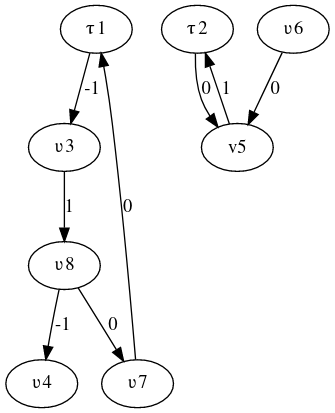
\includegraphics[width=0.3\linewidth]{images/digraph.png}
% Generating the graph requires \usepackage{dot2texi} or \usepackage[pdf]{graphviz}
\iffalse
\begin{dot2tex}[file=cstrnts,scale=0.6]
digraph D {
    t1 [label=<&tau;<SUB>1</SUB>>];
    t2 [label=<&tau;<SUB>2</SUB>>];
    v3 [label=<&upsilon;<SUB>3</SUB>>];
    v4 [label=<&upsilon;<SUB>4</SUB>>];
    v6 [label=<&upsilon;<SUB>6</SUB>>];
    v7 [label=<&upsilon;<SUB>7</SUB>>];
    v8 [label=<&upsilon;<SUB>8</SUB>>];
    v7 -> t1 [label="0"];
    v8 -> v7 [label="0"];
    t2 -> v5 [label="0"];
    v6 -> v5 [label="0"];
    v8 -> v4 [label="-1"];
    v3 -> v8 [label="1"];
    t1 -> v3 [label="-1"];
    v5 -> t2 [label="1"];
}
\end{dot2tex}
\fi
\caption{Example size variable constraints as a weighted directed graph}
\label{fig:digraph}
\end{figure}

%%% Local Variables:
%%% TeX-master: "../main.tex"
%%% TeX-engine: default
%%% End:


\RecCheckLoop then calls $\RecCheck(C, \tau_1, \set{\tau_1, \tau_2}, \upsilon_5)$.
Following its steps, we have:
\begin{enumerate}
    \item $V^\iota = \set{\upsilon_7, \upsilon_8, \upsilon_3}$, and we add the constraints $C' = \tau_1 \sqsubseteq V^\iota$ (subsizing each variable in $V^\iota$).
    \item It is evident that there are no negative-weight cycles in the constraint graph, so $V^- = \emptyset$.
    \item Nothing to be done.
    \item We have $\bigsqcup V^\neq = \set{\upsilon_5, \tau_2}$ and $\bigsqcup V^\iota = \set{\tau_1, \upsilon_3, \upsilon_8, \upsilon_7, \upsilon_4}$.
      Their intersection is empty, so we add no new constraints.
    \item There is no $\infty$ present, so $V^\bot = \emptyset$ and we return the constraints $C \cup C'$.
\end{enumerate}

\RecCheckLoop executes without failure, so \texttt{defBody} indeed has type $\text{Nat}^{\tau_1} \to \text{Nat}^{\tau_2}$.
Erasing this type to a global type for the global definition's type and to a position type for the fixpoint's type, the fully annotated program is then:

\begin{minted}[escapeinside=<>,mathescape=true]{coq}
Def example: Nat<$^\iota$> <$\to$> Nat<$^\iota$> <$\coloneqq$>
  fix<$_{\langle 1 \rangle, 1}$> <$\langle$>f: Nat<$^*$> <$\to$> Nat<$^*$> <$\coloneqq$>
    <$\lambda$>n: Nat. case<$_{\lambda x: \texttt{Nat}. \texttt{Nat}}$> n of
      <$\langle$>O <$\Rightarrow$> O,
       S <$\Rightarrow$> <$\lambda$>n': Nat. f n'<$\rangle \rangle$>.
\end{minted}
